\chapter{DỮ LIỆU VÀ PHƯƠNG PHÁP}
\label{ch:phuong_phap}

\section{Mô tả dữ liệu}

Đề tài dùng ba nguồn dữ liệu bổ trợ nhau. Nguyên tắc xuyên suốt khi lựa chọn là: \emph{mọi nhãn
dùng để chấm điểm đều phải có sẵn trong dữ liệu công khai}, không có con số nào phụ thuộc vào
việc tác giả tự gán nhãn cho hệ thống của chính mình. Bảng~\ref{tab:nguon_dulieu} tóm tắt ba
nguồn này.

\begin{table}[H]
\centering
\caption{Ba nguồn dữ liệu và vai trò của từng nguồn trong đề tài}
\label{tab:nguon_dulieu}
\small
\begin{tabularx}{\textwidth}{l l X}
\toprule
\textbf{Nguồn} & \textbf{Nhãn có sẵn} & \textbf{Vai trò trong đề tài} \\
\midrule
Cảnh tổng hợp & kích thước biết trước & thí nghiệm kiểm soát tỉ lệ và kiểm soát quan hệ \\
OCID & mặt nạ instance, độ sâu cảm biến & huấn luyện, đánh giá phân vùng, đếm, đo \\
COCO val2017 & mặt nạ và tên vật do người gán & đánh giá riêng phần nhận diện \\
\bottomrule
\end{tabularx}
\end{table}

\subsection{Bộ dữ liệu OCID}

OCID \cite{suchi2019ocid} gồm các chuỗi ảnh RGB-D chụp cảnh bàn và cảnh sàn với nhiều đồ vật đặt
lộn xộn, có che khuất. Mỗi khung hình đi kèm ảnh màu, ảnh độ sâu đã căn chỉnh (lưu ở đơn vị
milimet, hệ số quy đổi $0{,}001$ về mét) và ảnh nhãn instance. Bộ dữ liệu được tổ chức theo cây
thư mục phản ánh điều kiện chụp, mô tả ở Bảng~\ref{tab:ocid_cautruc}.

\begin{table}[H]
\centering
\caption{Cấu trúc phân cấp của bộ dữ liệu OCID}
\label{tab:ocid_cautruc}
\small
\begin{tabularx}{\textwidth}{l l X}
\toprule
\textbf{Cấp} & \textbf{Giá trị} & \textbf{Ý nghĩa} \\
\midrule
Nhóm vật    & ARID10, ARID20, YCB10 & bộ đồ vật dùng trong cảnh \\
Bề mặt      & table, floor          & vật đặt trên bàn hay trên sàn \\
Góc nhìn    & top, bottom           & máy ảnh nhìn từ cao hay ngang tầm \\
Chủng loại  & fruits, non-fruits, box, curved, mixed & đặc tính hình học của vật \\
Chuỗi cảnh  & seq01, seq05, \dots   & một cảnh, nhiều khung hình thêm dần vật \\
\bottomrule
\end{tabularx}
\end{table}

\subsubsection{Vấn đề rò rỉ dữ liệu và cách chia theo cảnh}

Điểm cần đặc biệt lưu ý khi dùng OCID là \emph{cách chia dữ liệu}. Các khung hình trong cùng một
chuỗi được ghi liên tiếp trong quá trình thêm dần đồ vật vào cảnh, nên hai khung hình liền kề
gần như giống hệt nhau. Nếu chia ngẫu nhiên theo khung hình, các ảnh gần trùng nhau sẽ xuất hiện
ở cả tập huấn luyện lẫn tập kiểm thử, khiến chỉ số mAP cao lên một cách giả tạo mà không phản
ánh khả năng khái quát thật. Hình~\ref{fig:split} minh hoạ hai cách chia.

\begin{figure}[H]
\centering
\begin{tikzpicture}[scale=0.9,font=\footnotesize]
  % ============ SAI: chia ngau nhien ============
  \node[anchor=west,font=\footnotesize\bfseries] at (0,3.3) {(a) Chia ngẫu nhiên theo khung hình --- RÒ RỈ};
  \foreach \i/\c in {0/black!15, 1/black!45, 2/black!15, 3/black!45, 4/black!15, 5/black!45} {
    \draw[fill=\c,draw=black!60] (\i*1.05, 2.3) rectangle (\i*1.05+0.9, 3.0);
  }
  \node[anchor=west,font=\scriptsize] at (6.5,2.65) {cùng một chuỗi \texttt{seq05}};
  \draw[decorate,decoration={brace,amplitude=4pt},thick] (0,2.15) -- (5.15,2.15);
  \node[font=\scriptsize,below] at (2.6,2.05) {các khung hình gần như giống hệt nhau};

  % ============ DUNG: chia theo chuoi ============
  \node[anchor=west,font=\footnotesize\bfseries] at (0,1.2) {(b) Chia theo chuỗi cảnh --- ĐÚNG};
  \foreach \i in {0,1,2} {
    \draw[fill=black!15,draw=black!60] (\i*1.05, 0.2) rectangle (\i*1.05+0.9, 0.9);
  }
  \foreach \i in {3,4,5} {
    \draw[fill=black!45,draw=black!60] (\i*1.05+0.5, 0.2) rectangle (\i*1.05+1.4, 0.9);
  }
  \draw[decorate,decoration={brace,amplitude=4pt},thick] (0,0.05) -- (2.85,0.05);
  \node[font=\scriptsize,below] at (1.4,-0.05) {\texttt{seq05} $\to$ huấn luyện};
  \draw[decorate,decoration={brace,amplitude=4pt},thick] (3.65,0.05) -- (6.65,0.05);
  \node[font=\scriptsize,below] at (5.15,-0.05) {\texttt{seq17} $\to$ kiểm thử};

  % chu thich mau
  \draw[fill=black!15,draw=black!60] (8.6,2.75) rectangle (9.1,3.05);
  \node[anchor=west,font=\scriptsize] at (9.2,2.9) {huấn luyện};
  \draw[fill=black!45,draw=black!60] (8.6,2.3) rectangle (9.1,2.6);
  \node[anchor=west,font=\scriptsize] at (9.2,2.45) {kiểm thử};
\end{tikzpicture}
\caption{Chia ngẫu nhiên theo khung hình gây rò rỉ dữ liệu; đề tài chia theo chuỗi cảnh}
\label{fig:split}
\end{figure}

Đề tài chia \emph{theo chuỗi cảnh} với hạt giống 42: toàn bộ khung hình của một chuỗi chỉ thuộc
về đúng một tập. Tập kiểm thử thu được gồm 26 chuỗi với 312 khung hình.

\subsection{Bộ dữ liệu COCO val2017}

Để đánh giá phần nhận diện trên ảnh đời thường, đề tài lấy 200 ảnh đầu tiên theo thứ tự tất định
từ tập COCO val2017 \cite{lin2014coco}. Bộ này có sẵn cả mặt nạ lẫn tên lớp do người gán, nên
cho phép chấm điểm nhận diện mà không tốn công gán nhãn.

Cần nhấn mạnh rằng ảnh COCO là ảnh đời thường (người, xe cộ, nội thất, cảnh đường phố), khác hẳn
phân bố của cảnh bàn OCID mà bộ phân vùng được huấn luyện. Đây là một lựa chọn \emph{có chủ ý}
nhằm đo khả năng khái quát ra ngoài miền huấn luyện, và cũng là lý do trực tiếp của tỉ lệ khớp
mặt nạ thấp báo cáo ở Chương~\ref{ch:ket_qua}.

\subsection{Cảnh tổng hợp}

Cảnh tổng hợp do đề tài tự sinh, gồm bốn vật với kích thước và vị trí biết trước hoàn toàn, kèm
bản đồ độ sâu đúng theo đơn vị mét. Cảnh tổng hợp không được dùng để báo cáo độ chính xác, vì mọi chỉ số đo trên dữ liệu có hình học biết trước đều đạt mức cao một cách hiển nhiên và không mang thông tin về năng lực thực tế. Vai trò của nó là thí nghiệm kiểm soát, xác nhận luồng xử lý hình học và các vị từ quan hệ được nối đúng trước khi áp dụng lên dữ liệu thật. Hình~\ref{fig:synth_scene} minh hoạ cảnh này qua các bước xử lý.

\begin{figure}[H]
\centering
\begin{subfigure}[b]{0.235\textwidth}
  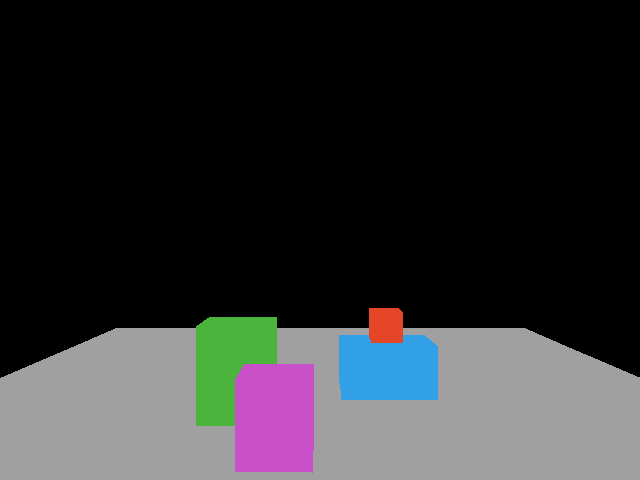
\includegraphics[width=\textwidth]{figures/synth_rgb.png}
  \caption{Ảnh màu}
\end{subfigure}
\hfill
\begin{subfigure}[b]{0.235\textwidth}
  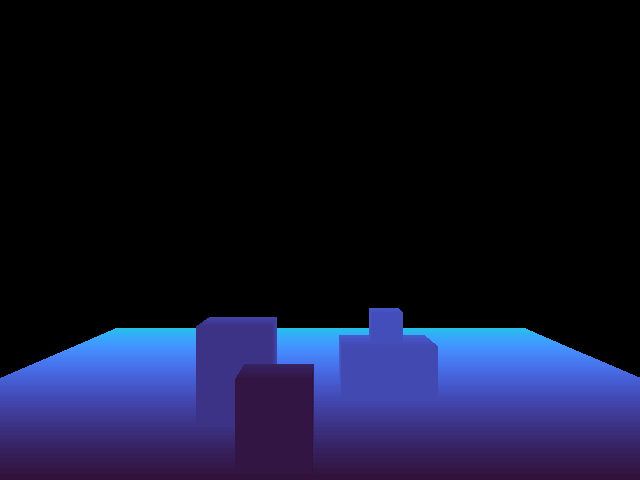
\includegraphics[width=\textwidth]{figures/synth_depth.png}
  \caption{Ảnh độ sâu}
\end{subfigure}
\hfill
\begin{subfigure}[b]{0.235\textwidth}
  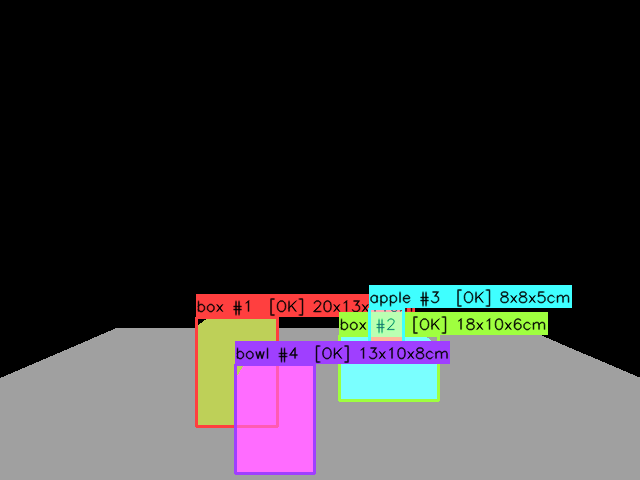
\includegraphics[width=\textwidth]{figures/synth_masks.png}
  \caption{Mặt nạ}
\end{subfigure}
\hfill
\begin{subfigure}[b]{0.235\textwidth}
  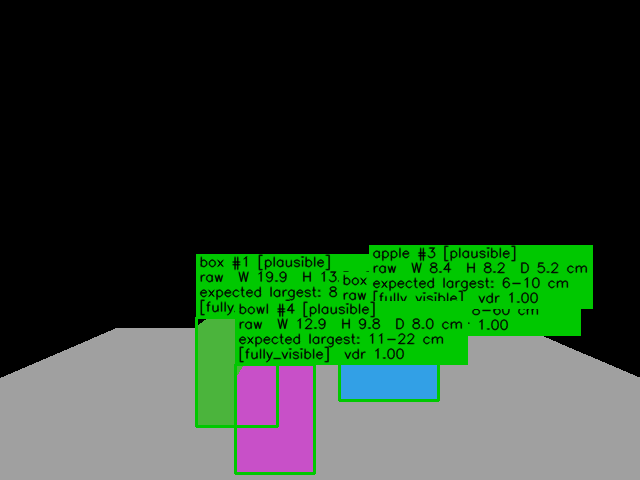
\includegraphics[width=\textwidth]{figures/synth_dimensions.png}
  \caption{Kích thước}
\end{subfigure}
\caption{Cảnh tổng hợp dùng làm thí nghiệm kiểm soát, với kích thước bốn vật biết trước}
\label{fig:synth_scene}
\end{figure}

\subsection{Hạn chế về tính đại diện của dữ liệu}

OCID chỉ chứa cảnh trong nhà, chụp bằng một loại cảm biến, với tập đồ vật hữu hạn đặt trên bàn
hoặc sàn. Kết quả phân vùng đạt được vì vậy \emph{không} suy rộng được cho cảnh ngoài trời, cho
cảm biến khác, hay cho các chủng loại vật không xuất hiện trong bộ dữ liệu. Tương tự, 200 ảnh
COCO là một mẫu nhỏ và các lớp phân bố rất lệch, nên độ chính xác nhận diện theo từng lớp có
khoảng tin cậy rộng. Cảnh tổng hợp thì hoàn toàn không mang tính đại diện cho thế giới thật; mọi
con số sinh ra từ nó chỉ được diễn giải như kiểm chứng phần mềm.

Hệ quả là các kết luận của đề tài bị giới hạn trong phạm vi: cảnh trong nhà, vật cứng không biến
dạng, bề mặt không trong suốt và không phản chiếu mạnh, có thông số nội máy ảnh.

\section{Tiền xử lý}

Các bước tiền xử lý được thực hiện theo đúng thứ tự sau.

\begin{enumerate}[leftmargin=1.5cm]
\item \textbf{Chuẩn hoá đơn vị độ sâu.} Nhân giá trị độ sâu thô với hệ số $0{,}001$ để quy về
mét, tương ứng với quy ước lưu trữ milimet của OCID.
\item \textbf{Loại giá trị không hợp lệ.} Bỏ các điểm ảnh có độ sâu bằng không (cảm biến không
đo được), nhỏ hơn $0{,}1$~m hoặc lớn hơn $5{,}0$~m --- các ngưỡng này loại phần lớn nhiễu cảm
biến mà vẫn bao trọn khoảng làm việc của cảnh bàn.
\item \textbf{Tách mặt phẳng nền bằng RANSAC.} Ước lượng mặt phẳng bàn hoặc sàn với ngưỡng khoảng
cách $0{,}01$~m rồi loại các điểm thuộc mặt phẳng đó, tránh việc mặt bàn bị gộp vào đám mây điểm của vật và làm hộp bao mở rộng quá mức.
\item \textbf{Lọc ngoại lai thống kê.} Với mỗi điểm, xét 20 điểm lân cận gần nhất và loại các
điểm có khoảng cách trung bình vượt quá 2 lần độ lệch chuẩn của toàn tập.
\item \textbf{Chuyển đổi định dạng nhãn.} Ảnh nhãn instance của OCID được chuyển sang định dạng
đa giác của YOLO để huấn luyện, và sang định dạng COCO để đánh giá bằng \texttt{pycocotools}.
\end{enumerate}

\section{Kiến trúc hệ thống đề xuất}

Hệ thống gồm tám bước nối tiếp, dùng chung một luồng mã nguồn cho cả chế độ dòng lệnh lẫn ứng
dụng web nhằm đảm bảo kết quả nhất quán. Hình~\ref{fig:pipeline} trình bày sơ đồ tổng thể.

\begin{figure}[H]
\centering
\begin{tikzpicture}[
  font=\scriptsize,
  box/.style={draw=black!70,fill=black!6,rounded corners=2pt,minimum width=2.05cm,
              minimum height=0.85cm,align=center,inner sep=2pt},
  newbox/.style={box,fill=black!22,draw=black,thick},
  io/.style={draw=black!70,fill=white,rounded corners=2pt,minimum width=3.0cm,
             minimum height=0.8cm,align=center,inner sep=2pt},
  ar/.style={->,>=Stealth,black!70,thick}
]
% --- dau vao ---
\node[io] (in) at (0,3.0) {Ảnh RGB\\ (+ độ sâu, thông số nội)};

% --- hang 1 ---
\node[box] (b1) at (3.4,3.0) {\textbf{1.} Tiền xử lý\\ độ sâu};
\node[box] (b2) at (6.1,3.0) {\textbf{2.} Phân vùng\\ YOLO-seg};
\node[box] (b3) at (8.8,3.0) {\textbf{3.} Đếm\\ hai tầng lọc};
\node[box] (b4) at (11.5,3.0) {\textbf{4.} Đo 3D\\ (OBB)};

\draw[ar] (in) -- (b1);
\draw[ar] (b1) -- (b2);
\draw[ar] (b2) -- (b3);
\draw[ar] (b3) -- (b4);

% --- xuong hang 2 ---
\draw[ar] (b4.south) -- ++(0,-0.55) -| (11.5,1.6);

% --- hang 2 (nguoc chieu) ---
\node[newbox] (b5) at (11.5,1.15) {\textbf{5.} Nhận diện\\ CLIP + từ chối};
\node[newbox] (b6) at (8.8,1.15) {\textbf{6.} Kiểm tra\\ tính hợp lý};
\node[newbox] (b7) at (6.1,1.15) {\textbf{7.} Hiệu chỉnh\\ tỉ lệ};
\node[box]    (b8) at (3.4,1.15) {\textbf{8.} Quan hệ\\ không gian};
\node[io]     (out) at (0,1.15) {Đồ thị cảnh\\ JSON + hình};

\draw[ar] (b5) -- (b6);
\draw[ar] (b6) -- (b7);
\draw[ar] (b7) -- (b8);
\draw[ar] (b8) -- (out);

% --- tri thuc kich thuoc ---
\node[draw=black!70,fill=white,rounded corners=2pt,align=center,
      minimum width=2.6cm,minimum height=0.7cm] (kb) at (10.15,-0.35)
      {Bảng tri thức kích thước\\ (\texttt{object\_priors.yaml})};
\draw[ar,dashed] (kb.north) -- ++(0,0.25) -| (b5.south);
\draw[ar,dashed] (kb) -- (b6.south);
\draw[ar,dashed] (kb.west) -- ++(-0.4,0) |- (b7.south);

% --- chu thich ---
\node[newbox,minimum width=0.7cm,minimum height=0.4cm] at (1.1,-0.35) {};
\node[anchor=west,font=\scriptsize] at (1.55,-0.35) {ba bước bổ sung ở giai đoạn hai};
\end{tikzpicture}
\caption{Kiến trúc tám bước của hệ thống; ba bước tô đậm là đóng góp chính của đề tài}
\label{fig:pipeline}
\end{figure}

\subsection{Bước 2--3: Phân vùng và đếm hai tầng}

Bước phân vùng dùng YOLOv8n-seg \cite{jocher2023yolov8} huấn luyện lại với đúng một lớp
\texttt{object}. Bước đếm áp dụng hai tầng lọc nối tiếp, mô tả ở Bảng~\ref{tab:hai_tang}.

\begin{table}[H]
\centering
\caption{Hai tầng lọc trong bước đếm đối tượng}
\label{tab:hai_tang}
\small
\begin{tabularx}{\textwidth}{l l X}
\toprule
\textbf{Tầng} & \textbf{Nguồn tin} & \textbf{Tiêu chí loại bỏ} \\
\midrule
Tầng 1 & chỉ ảnh màu
  & điểm tin cậy $< 0{,}25$; diện tích $< 200$ điểm ảnh; trùng lặp NMS ở IoU $> 0{,}8$ \\
\addlinespace
Tầng 2 & thông tin độ sâu
  & tỉ lệ điểm ảnh có độ sâu hợp lệ $< 0{,}2$; số điểm ba chiều $< 100$ \\
\bottomrule
\end{tabularx}
\end{table}

Việc tách rời hai tầng cho phép đo trực tiếp phần đóng góp riêng của độ sâu bằng cách bật hoặc
tắt tầng thứ hai --- đây chính là thí nghiệm loại trừ trả lời Câu hỏi nghiên cứu 1.1.

\subsection{Bước 5: Nhận diện từ vựng mở có cơ chế từ chối}
\label{sec:tuchoi}

Bộ nhận diện cắt vùng ảnh quanh mỗi mặt nạ với phần đệm ngữ cảnh 10\%, làm mờ nền thay vì xoá
hẳn (hệ số $0{,}55$) để giữ lại manh mối ngữ cảnh, rồi đưa qua CLIP ViT-B/32
\cite{radford2021clip,ilharco2021openclip}. Ba đặc điểm thiết kế quan trọng:

\begin{itemize}[leftmargin=1.5cm]
\item \textbf{Từ vựng sinh từ bảng tri thức kích thước.} Danh sách lớp không được viết tay riêng
mà lấy trực tiếp từ tệp cấu hình chứa dải kích thước (87 lớp cùng một số nhãn phi vật thể
đóng vai trò gây nhiễu). Nhờ vậy bộ nhận diện chỉ có thể phát ra những tên mà hệ thống thực sự
có tri thức kích thước tương ứng, và hai thành phần không thể lệch nhau theo thời gian.
\item \textbf{Gộp mẫu câu.} Theo Công thức~\eqref{eq:prompt_ens} với $M = 7$ cách diễn đạt, tính
một lần khi nạp mô hình.
\item \textbf{Cơ chế từ chối ba tiêu chí.} Chi tiết ở Bảng~\ref{tab:tu_choi}.
\end{itemize}

\begin{table}[H]
\centering
\caption{Ba tiêu chí kích hoạt cơ chế từ chối, trả về nhãn \texttt{unknown}}
\label{tab:tu_choi}
\small
\begin{tabularx}{\textwidth}{l l X}
\toprule
\textbf{Tiêu chí} & \textbf{Ngưỡng} & \textbf{Lý do} \\
\midrule
Điểm số tuyệt đối & $< 0{,}30$
  & mô hình không tự tin ở bất kỳ lớp nào \\
Khoảng cách hạng nhất--nhì & $< 0{,}05$
  & hai lớp ngang nhau, lựa chọn gần như ngẫu nhiên \\
Lớp thắng là nhãn phi vật thể & ---
  & vùng cắt thực chất là nền (\texttt{background}, \texttt{wall}\dots) \\
\bottomrule
\end{tabularx}
\end{table}

Điểm cần nhấn mạnh: Vật bị từ chối vẫn được đo kích thước như bình thường, nhưng không tham gia vào tập bỏ phiếu ở bước hiệu chỉnh. Thiết kế này tách bạch hai chức năng: phép đo không phụ thuộc vào danh tính vật, trong khi phép hiệu chỉnh thì có. Thiết kế này tách bạch hai chức năng --- đo lường không cần biết tên
vật, còn hiệu chỉnh thì cần.

\subsection{Bước 6: Tri thức kích thước và kiểm tra tính hợp lý}

Mỗi lớp trong bảng tri thức lưu một khoảng $[\min, \max]$ cho từng chiều trong ba chiều đã sắp
giảm dần, cùng một giá trị neo \texttt{scale\_anchor\_cm} là cạnh dài nhất điển hình của lớp đó.
Bảng~\ref{tab:vidu_prior} nêu vài ví dụ minh hoạ.

\begin{table}[H]
\centering
\caption{Ví dụ một số mục trong bảng tri thức kích thước (đơn vị: cm)}
\label{tab:vidu_prior}
\small
\begin{tabular}{lccc}
\toprule
\textbf{Lớp} & \textbf{Chiều dài nhất} & \textbf{Chiều thứ hai} & \textbf{Neo tỉ lệ} \\
\midrule
apple   & $[6{,}0;\ 10{,}0]$  & $[6{,}0;\ 9{,}0]$   & $8{,}0$ \\
cup     & $[7{,}0;\ 15{,}0]$  & $[6{,}0;\ 12{,}0]$  & $10{,}0$ \\
laptop  & $[28{,}0;\ 42{,}0]$ & $[20{,}0;\ 30{,}0]$ & $35{,}0$ \\
chair   & $[70{,}0;\ 110{,}0]$& $[40{,}0;\ 60{,}0]$ & $90{,}0$ \\
\bottomrule
\end{tabular}
\end{table}

Các khoảng được đặt rộng rãi có chủ ý, vì mục tiêu là phát hiện sai lệch thô, không nhằm phân biệt những sai khác tự nhiên giữa các cá thể trong cùng một lớp. Kết quả so sánh sinh ra kết luận hợp lý hoặc không hợp lý
cho từng chiều và cho cả vật, hiển thị đồng nhất ở mọi đầu ra.

\subsection{Bước 7: Hiệu chỉnh tỉ lệ toàn ảnh}
\label{sec:calib}

Xuất phát từ Công thức~\eqref{eq:scale_assume} ở Chương~\ref{ch:co_so} rằng độ sâu đơn mắt chỉ
sai khác một hệ số nhân duy nhất cho cả ảnh, đề tài ước lượng đúng một hệ số $s$ cho mỗi ảnh
thay vì sửa từng vật riêng lẻ. Cách sửa từng vật theo tri thức tiên nghiệm của riêng nó ---
phương án trực giác và cũng là phương án phiên bản trước của đề tài từng dùng --- vừa thiếu ràng
buộc vừa mang tính vòng tròn như đã phân tích ở Mục~\ref{sec:vongtron}.

Mỗi vật $i$ đủ điều kiện đóng góp một lá phiếu theo Công thức~\eqref{eq:vote}, trong đó $a_i$ là
giá trị neo của lớp được nhận diện và $d_i$ là cạnh dài nhất đo được.

\begin{equation}
\label{eq:vote}
r_i = \frac{a_i}{d_i}
\end{equation}

Hệ số tỉ lệ của cả ảnh là trung vị của tập phiếu, theo Công thức~\eqref{eq:median}, với $V$ là
tập chỉ số các vật đủ điều kiện bỏ phiếu. Việc dùng trung vị thay vì trung bình khiến một vật bị
gán nhãn sai không thể kéo lệch ước lượng.

\begin{equation}
\label{eq:median}
s = \operatorname{median}\{\, r_i : i \in V \,\}
\end{equation}

Hệ số $s$ sau đó nhân vào kích thước của \emph{mọi} vật trong ảnh, kể cả những vật không bỏ
phiếu và những vật không rõ danh tính --- đây là điểm khác biệt cốt lõi so với cách sửa từng
vật. Giá trị đo gốc không bao giờ bị ghi đè; kết quả sau hiệu chỉnh được lưu ở trường riêng để
cả hai luôn hiển thị cạnh nhau.

Độ phân tán của tập phiếu được đo bằng độ lệch tuyệt đối trung vị tương đối theo
Công thức~\eqref{eq:mad}. Khi đại lượng này vượt ngưỡng, các phiếu được coi là bất đồng và hệ
thống từ chối hiệu chỉnh.

\begin{equation}
\label{eq:mad}
\mathrm{relMAD}(V) = \frac{\operatorname{median}\{\, |r_i - s| : i \in V \,\}}{s}
\end{equation}

Thuật toán~\ref{alg:calib} trình bày đầy đủ các điều kiện loại phiếu và hai chốt an toàn.

% Đổi nhãn float sang tiếng Việt cho khớp với phần còn lại của báo cáo.
% (Gói `algorithm` đặt mặc định là "Algorithm"; template không renew nhãn này.)
\floatname{algorithm}{Thuật toán}

\begin{algorithm}[H]
\caption{Hiệu chỉnh tỉ lệ toàn ảnh theo bỏ phiếu trung vị}
\label{alg:calib}
\begin{algorithmic}[1]
\State \textbf{Đầu vào:} tập vật $O$ với nhãn, điểm số, kích thước đo được; bảng tri thức $P$
\State \textbf{Đầu ra:} hệ số tỉ lệ $s$ và cờ quyết định có áp dụng hay không
\State $V \gets \emptyset$
\For{mỗi vật $o \in O$}
    \If{$o$ là \texttt{unknown} \textbf{hoặc} điểm số $< 0{,}30$}
        \State \textbf{continue} \Comment{nhãn không đáng tin}
    \EndIf
    \If{lớp của $o$ có kích thước quá biến thiên}
        \State \textbf{continue} \Comment{ví dụ: hộp, bát, chậu cây}
    \EndIf
    \If{$o$ bị cắt bởi mép ảnh}
        \State \textbf{continue} \Comment{vật bị cắt đo ngắn, làm lệch tỉ lệ lên cao}
    \EndIf
    \If{tỉ lệ hình dạng đo được lệch quá 2 lần so với lớp}
        \State \textbf{continue} \Comment{sai tỉ lệ đồng nhất phải bảo toàn hình dạng}
    \EndIf
    \State $V \gets V \cup \{\, a_o / d_o \,\}$
\EndFor
\If{$|V| = 0$}
    \State \Return $s = 1$, không áp dụng
\EndIf
\State $s \gets \operatorname{median}(V)$
\If{$s \in [0{,}9;\ 1{,}1]$}
    \State \Return $s$, không áp dụng \Comment{vùng chết: tỉ lệ vốn đã đúng}
\EndIf
\If{$\mathrm{relMAD}(V) > 0{,}6$}
    \State \Return $s$, không áp dụng \Comment{chốt 1: các phiếu bất đồng}
\EndIf
\If{nhân $s$ làm giảm số vật nằm trong dải hợp lý}
    \State \Return $s$, không áp dụng \Comment{chốt 2: hiệu chỉnh làm xấu đi}
\EndIf
\State \Return $s$, áp dụng cho mọi vật
\end{algorithmic}
\end{algorithm}

\subsection{Bước 8: Suy luận quan hệ không gian và đồ thị cảnh}

Bước cuối xét từng cặp vật và phát ra các vị từ có hướng dựa trên luật hình học, mô tả ở
Bảng~\ref{tab:vitu}.

\begin{table}[H]
\centering
\caption{Tập vị từ quan hệ không gian và điều kiện kích hoạt}
\label{tab:vitu}
\small
\begin{tabularx}{\textwidth}{l X}
\toprule
\textbf{Vị từ} & \textbf{Điều kiện} \\
\midrule
\texttt{in\_front\_of} / \texttt{behind}
  & hiệu độ sâu trung vị của hai vật vượt $0{,}02$~m \\
\texttt{overlaps}
  & IoU khung bao hai chiều vượt $0{,}05$ \\
\texttt{occludes} / \texttt{partially\_occluded\_by}
  & mức chồng lấn vượt $0{,}15$ kèm thứ tự độ sâu rõ ràng \\
\texttt{likely\_on\_top\_of}
  & tâm vật chủ thể nằm ở $40\%$ trên của vùng hợp, chồng lấn ngang $> 0{,}2$,
    chênh lệch độ sâu $< 0{,}08$~m \\
\bottomrule
\end{tabularx}
\end{table}

Toàn bộ kết quả được đóng gói thành đồ thị cảnh dạng JSON theo tinh thần của
\cite{johnson2015scenegraph}, kèm các cờ độ tin cậy như mức độ nhìn thấy và tỉ lệ điểm ảnh có độ
sâu hợp lệ, để hệ thống phía sau biết được kết quả đáng tin tới đâu.

\section{Chỉ số đánh giá}

\subsection{Đếm đối tượng}

Với $n$ khung hình, gọi $\hat{c}_k$ và $c_k$ lần lượt là số vật dự đoán và số vật thật của khung
hình $k$. Sai số tuyệt đối trung bình và tỉ lệ đếm đúng tuyệt đối cho bởi
Công thức~\eqref{eq:mae} và \eqref{eq:exact}.

\begin{equation}
\label{eq:mae}
\mathrm{MAE} = \frac{1}{n}\sum_{k=1}^{n} \left| \hat{c}_k - c_k \right|
\end{equation}

\begin{equation}
\label{eq:exact}
\mathrm{Acc}_{\text{exact}} = \frac{1}{n}\sum_{k=1}^{n} \mathbf{1}\!\left[\hat{c}_k = c_k\right]
\end{equation}

Số vật thật được định nghĩa là số mặt nạ instance của OCID có diện tích từ 200 điểm ảnh trở lên,
khớp đúng với ngưỡng diện tích tối thiểu mà hệ thống dùng khi lọc --- nếu không thống nhất hai
ngưỡng này, hệ thống sẽ bị phạt oan vì bỏ qua đúng những vật mà nó được cấu hình để bỏ qua.

\subsection{Nhận diện}

Đề tài báo cáo hai nhóm chỉ số tách bạch để tránh nhập nhằng. Nhóm thứ nhất tính \emph{trên các
mặt nạ đã khớp}: mặt nạ dự đoán được ghép một-một với mặt nạ thật theo IoU tham lam ở ngưỡng
$0{,}5$, sau đó tính top-1, top-3, tỉ lệ từ chối và độ chính xác top-1 khi mô hình đã quyết định
đưa ra nhãn. Nhóm thứ hai là chỉ số \emph{đầu-cuối}, nhân thêm tỉ lệ khớp mặt nạ, theo
Công thức~\eqref{eq:e2e}.

\begin{equation}
\label{eq:e2e}
\mathrm{Acc}_{\text{đầu-cuối}} = \mathrm{Acc}_{\text{top-1}} \times \mathrm{MatchRate}
\end{equation}

Chỉ số nhóm thứ nhất \emph{không được phép} trình bày như độ chính xác của cả hệ thống; báo cáo
luôn đặt hai con số cạnh nhau.

\subsection{Đo kích thước và thủ tục để-lại-một}
\label{sec:loo}

Đây là phần thiết kế thực nghiệm quan trọng nhất của đề tài. Mỗi vật được đo \emph{hai lần từ
cùng một khung hình với cùng một mặt nạ thật}, chỉ thay đổi nguồn độ sâu. Hình~\ref{fig:loo}
minh hoạ thiết kế này.

\begin{figure}[H]
\centering
\begin{tikzpicture}[
  font=\scriptsize,
  b/.style={draw=black!70,fill=black!6,rounded corners=2pt,minimum width=2.5cm,
            minimum height=0.75cm,align=center,inner sep=2pt},
  ar/.style={->,>=Stealth,black!70,thick}
]
\node[b] (frame) at (0,1.1) {Một khung hình OCID\\ + mặt nạ THẬT};

\node[b] (sensor) at (3.9,2.15) {Độ sâu cảm biến};
\node[b] (midas)  at (3.9,0.05) {Độ sâu MiDaS};

\node[b] (ref)  at (7.6,2.15) {Kích thước\\ THAM CHIẾU};
\node[b] (pred) at (7.6,0.05) {Kích thước\\ DỰ ĐOÁN};

\node[b,fill=black!22,draw=black,thick] (calib) at (11.2,0.05)
  {Hiệu chỉnh bằng\\ hệ số từ CÁC VẬT KHÁC};

\draw[ar] (frame.east) -- ++(0.35,0) |- (sensor.west);
\draw[ar] (frame.east) -- ++(0.35,0) |- (midas.west);
\draw[ar] (sensor) -- (ref);
\draw[ar] (midas)  -- (pred);
\draw[ar] (pred)   -- (calib);

\draw[<->,>=Stealth,thick,black] (ref.south) -- node[right,font=\scriptsize]{so sánh} (pred.north);
\draw[<->,>=Stealth,thick,black,dashed] (calib.north) -- ++(0,1.4) -| (ref.east);
\end{tikzpicture}
\caption{Thiết kế đo hai lần cùng mặt nạ: chỉ nguồn độ sâu thay đổi, nên chất lượng phân vùng
không phải biến gây nhiễu}
\label{fig:loo}
\end{figure}

Vì cả hai nhánh dùng chung mặt nạ thật, chất lượng phân vùng bị loại khỏi vai trò biến gây
nhiễu. Vì cả hai cùng đo \emph{phần nhìn thấy}, không có sai lệch hệ thống giữa hai đại lượng
được so sánh --- đây chính là lý do đề tài không dùng kích thước CAD từ BOP \cite{hodan2018bop}
hay YCB \cite{calli2015ycb} làm tham chiếu.

Để phá vỡ tính vòng tròn, hệ số tỉ lệ dùng để hiệu chỉnh vật $j$ được ước lượng từ \emph{toàn bộ
các vật còn lại} trong ảnh, loại trừ hoàn toàn $j$ khỏi cả lá phiếu lẫn chốt kiểm tra tính nhất
quán hậu nghiệm. Chỉ số báo cáo là MAE trước và sau hiệu chỉnh cùng mức thay đổi tương đối theo
Công thức~\eqref{eq:improve}.

\begin{equation}
\label{eq:improve}
\Delta = \frac{\mathrm{MAE}_{\text{sau}} - \mathrm{MAE}_{\text{trước}}}{\mathrm{MAE}_{\text{trước}}} \times 100\%
\end{equation}

Một quy ước quan trọng: khi hệ thống quyết định \emph{không} hiệu chỉnh (rơi vào vùng chết hoặc
bị một trong hai chốt chặn), vật đó được tính là phép đo không đổi chứ không bị loại khỏi mẫu số.
Nếu chỉ số sẽ bị thổi phồng vì chỉ còn giữ lại các trường hợp thuận lợi.

\subsection{Quan hệ không gian}

Bài toán quan hệ là đa nhãn trên từng cặp có hướng, nên đề tài báo cáo độ chính xác trùng khớp
toàn tập nhãn cho mỗi cặp, cùng các chỉ số $F_1$ vi mô và vĩ mô theo từng loại quan hệ.

\section{Thiết lập thực nghiệm}

Bảng~\ref{tab:thiet_lap} liệt kê cấu hình đã dùng để sinh ra toàn bộ kết quả trong
Chương~\ref{ch:ket_qua}. Toàn bộ con số được tạo từ đúng một tệp trọng số duy nhất, có mã băm
SHA-256 ghi trong bảng, và không có lần chạy nào dùng mô hình dự phòng.

\begin{table}[H]
\centering
\caption{Cấu hình thực nghiệm và thông tin xác thực trọng số}
\label{tab:thiet_lap}
\small
\begin{tabularx}{\textwidth}{l X}
\toprule
\textbf{Hạng mục} & \textbf{Giá trị} \\
\midrule
Kiến trúc phân vùng & YOLOv8n-seg, một lớp \texttt{object} \\
Huấn luyện          & 100 epoch, kích thước ảnh 640, batch 8, hạt giống 42 \\
Mã băm SHA-256      & {\footnotesize\texttt{152a8923e81d14d3a90a9204c4be17bc76de5c1a5caf1845cb423a7c0cafd771}} \\
Dùng mô hình dự phòng & không \\
Mô hình nhận diện   & CLIP ViT-B/32, trọng số \texttt{openai} \\
Độ sâu đơn mắt      & MiDaS (backbone qua thư viện \texttt{timm}) \\
Khung học sâu       & PyTorch 2.8.0 \cite{paszke2019pytorch} \\
Xử lý ảnh / 3D      & OpenCV 4.13 \cite{bradski2000opencv}, Open3D 0.18 \cite{zhou2018open3d} \\
Ngôn ngữ            & Python 3.11 \\
Kiểm thử tự động    & 74 kiểm thử, chạy được không cần tải mô hình \\
\bottomrule
\end{tabularx}
\end{table}

Các siêu tham số quan trọng của bước hiệu chỉnh được trình bày ở Mã nguồn~\ref{lst:calib_cfg}.

\begin{lstlisting}[language=Python,caption={Cấu hình bước hiệu chỉnh tỉ lệ},label={lst:calib_cfg}]
calibration = {
    "enabled": True,
    "min_label_score": 0.30,        # chi tin cac nhan du tin cay
    "min_votes": 1,                 # 1 cho phep anh chi co mot vat
    "min_valid_depth_ratio": 0.3,   # vat bo phieu phai co du diem do sau
    "exclude_truncated": True,      # vat bi cat boi mep anh do ngan
    "max_aspect_mismatch": 2.0,     # hinh dang phai giong lop duoc nhan dien
    "deadband_low": 0.9,            # trong [low, high] coi nhu ti le da dung
    "deadband_high": 1.1,
    "max_rel_mad": 0.6,             # chot 1: cac phieu bat dong
    "verify_improves_consistency": True,   # chot 2: khong duoc lam xau di
}
\end{lstlisting}
